\chapter{Learning Prob. Submodular Models} \label{ch:genes}

\section{Introduction}
As discussed at the very beginning of the thesis, learning probabilistic models from data in one of our main motivations.
The probabilistic framework we employ suggests a principled way to estimate the model parameters given a data set, namely by maximizing the model likelihood under the data.
Unfortunately, the maximum likelihood problem for the model class we consider is, in general, non-convex; even worse, evaluating the likelihood function or its gradient with respect to the model parameters boils down to computing expectations over the distribution at hand, which we have already seen to be a hard problem.
We show in this chapter how we can use sampling to approximate the likelihood gradients, and, thus, perform an approximate gradient ascent procedure that converges to a local optimum of the model likelihood.
Then, we focus on applying this learning procedure to the application of modeling the interactions between gene alterations in cancer patients.
We evaluate our method on synthetic and real cancer data, visualize the results in several ways, and compare them to previously proposed statistical methods.


\section{Approximate Maximum Likelihood Learning using Sampling}

As before, we consider a model of the form
\begin{align*}
p(S; \btheta) = \frac{1}{Z(\btheta)} \exp\left( F(S; \btheta) \right),
\end{align*}
parametrized by a vector $\btheta$, which we would like to learn.
Given a data set of $N$ sets, $\mathcal{D} \defeq (D_1,\ldots,D_N)$, $D_1,\ldots,D_N \subseteq V$, the log-likelihood of the model is
\begin{align*}
\ell(\btheta) &\defeq \sum_{i=1}^N \log p(D_i; \btheta)\\
           &= \sum_{i=1}^N \left( F(D_i; \btheta) - \log Z(\btheta) \right)\\
           &= \sum_{i=1}^N F(D_i; \btheta) - N \log Z(\btheta).
\end{align*}
The gradient of the log-likelihood with respect to the parameters $\btheta$ is
\begin{align*}
                 \*g(\btheta) &\defeq \nabla_{\btheta} \ell(\btheta)\\
                              &= \sum_{i=1}^N \nabla_{\btheta} F(D_i; \btheta) - N \nabla_{\btheta} \log Z(\btheta)\\
                              &= \sum_{i=1}^N \nabla_{\btheta} F(D_i; \btheta) - N \frac{1}{Z(\btheta)} \nabla_{\btheta} Z(\btheta)\\
                              &= \sum_{i=1}^N \nabla_{\btheta} F(D_i; \btheta) - N \frac{1}{Z(\btheta)} \nabla_{\btheta} \sum_{S \subseteq V} \exp\left( F(S; \btheta) \right)\\
                              &= \sum_{i=1}^N \nabla_{\btheta} F(D_i; \btheta) - N \sum_{S \subseteq V} \frac{\exp\left( F(S; \btheta)\right)}{Z(\btheta)} \nabla_{\btheta} F(S; \btheta)\\
                              &= \sum_{i=1}^N \nabla_{\btheta} F(D_i; \btheta) - N \sum_{S \subseteq V} p(S; \btheta) \nabla_{\btheta} F(S; \btheta)\\
                              &= \sum_{i=1}^N \nabla_{\btheta} F(D_i; \btheta) - N\,\E_{p}\left[ \nabla_{\btheta} F(S; \btheta) \right]\\
                              &= \frac{1}{N}\sum_{i=1}^N \nabla_{\btheta} F(D_i; \btheta) - \E_{p}\left[ \nabla_{\btheta} F(S; \btheta) \right].
\end{align*}
This shows that the maximum likelihood parameters satisfy a generalized version of the well-known moment matching condition for exponential family models; cf. \cite[Ch. 20]{koller09}.
That is, at the maximum, the empirical mean of the function gradient over the data set will match the expected gradient over the model distribution.

While the expectation term in the log-likelihood gradient is, in general, infeasible to compute exactly, we can straightforwardly approximate it using the sampling methods discussed in the previous chapters.
In particular, if we have drawn samples $\mathcal{S} = \{ S_1,\ldots,S_M \}$, $S_1,\ldots,S_M \subseteq V$, from distribution $p$, we can approximate the gradient $\*g(\btheta)$ by
\begin{align*}
\widetilde{\*g}(\btheta) \defeq \frac{1}{N}\sum_{i=1}^N \nabla_{\btheta} F(D_i; \btheta) - \frac{1}{M}\sum_{i=1}^M \nabla_{\btheta} F(S_i; \btheta).
\end{align*}
We, therefore, propose learning the parameters $\btheta$ using an approximate gradient ascent procedure, which involves alternating between sampling from the current model to compute $\widetilde{\*g}(\btheta)$, and performing a gradient step towards the direction of $\widetilde{\*g}(\btheta)$, as shown in \algoref{alg:grad}.

\begin{algorithm}[tb]
  \setstretch{1.2}
  \caption{Approximate maximum likelihood maximization}
  \label{alg:grad}
    \begin{algorithmic}[1]
      \REQUIRE Data $\mathcal{D}$, iterations $n_{\mathrm{iter}}$, samples $M$, step $(\gamma_i)_i$, gradient oracle $\nabla_{\btheta} F(S; \btheta)$
      \STATE Initialize $\theta$
      \FOR{$i = 1$ \TO $n_{\mathrm{iter}}$}
        \LET{$\mathcal{S}$}{sample $M$ sets from $p(\cdot\,; \theta)$}
        \LET{$\widetilde{\*g}(\btheta)$}{$\frac{1}{N}\sum_{i=1}^N \nabla_{\btheta} F(D_i; \btheta) - \frac{1}{M}\sum_{i=1}^M \nabla_{\btheta} F(S_i; \btheta)$}
        \LET{$\btheta$}{$\btheta + \gamma_i\,\widetilde{\*g}(\btheta)$}
      \ENDFOR
      \RETURN $\btheta$
    \end{algorithmic}
\end{algorithm}

\paragraph{Gradients of the \fldc{} model.}
Since we will be focusing on the \fldc{} model for the remainder of this chapter, we derive here the gradients of its potential function with respect to its parameters.
For simplicity, we assume that we use an equal number of $L$ dimensions for both the repulsive and the attractive matrices.
As a reminder, the \fldc{} model is then defined via the following potential \citep{djolonga16mixed},
\begin{align*}
F(S; \bu, \bw, \bv) = \sum_{i \in S} u_i + \sum_{j=1}^{L} \left(\max_{i \in S} w_{ij} - \sum_{i \in S} w_{ij}\right) - \sum_{j=1}^{L} \left(\max_{i \in S} v_{ij} - \sum_{i \in S} v_{ij}\right).
\end{align*}
$F$ is differentiable almost everywhere, due to the presence of the two ``$\max$'' functions.
For the points where it is not differentiable, we define subgradients that give equal contribution to all elements that belong to the corresponding ``$\argmax$''.
In particular, for all $i \in V$, $j \in [L]$, we have
\begin{align*}
\nabla_{u_i} F(S; \bu, \bw, \bv) &= \ind[i \in S]\\
\nabla_{w_{ij}} F(S; \bu, \bw, \bv) &= \frac{\ind[i \in \argmax_{r \in S} w_{rj}]}{|\argmax_{r \in S} w_{rj}|} - \ind[i \in S]\\
\nabla_{v_{ij}} F(S; \bu, \bw, \bv) &= -\frac{\ind[i \in \argmax_{r \in S} v_{rj}]}{|\argmax_{r \in S} v_{rj}|} + \ind[i \in S].
\end{align*}
\citet{tschiatschek16} used an alternative set of subgradients, involving randomization over the choice of the ``$\argmax$'' at each gradient step.
We have noticed that our choice often results in slightly improved learning performance in practice.


\paragraph{Implementation details.}
By definition of the \fldc{} model, the elements of matrices $\bw$ and $\bv$ must be non-negative.
To achieve this during learning, we project the entries of $\bw$ and $\bv$ to the positive orthant after each gradient step.

Furthermore, we have found it beneficial in practice to induce sparsity on these matrices, in order to reduce the effect of noisy data on the learned models, and obtain more interpretable solutions.
To this end, we employ an $L_1$ regularization to both $\bw$ and $\bv$ by projecting each row and column of this matrices to the corresponding $L_1$-ball after each gradient step.

We initialize the entries of $\bu$ to the maximum likelihood estimates of the respective product distribution, that is,
\begin{align*}
u_i = \log\left( \frac{f_i}{1 - f_i} \right),
\end{align*}
where $f_i$ is the frequency of element $i \in V$ in the data set $\mathcal{D}$.
We randomly initialize the entries of $\bw$ and $\bv$ by drawing from a uniform distribution $\mathcal{U}[0, 0.01]$.
Finally, we use a fixed step size ($\gamma = 5e^{-4}$) for the first half of the iterations, and a geometrically decreasing step size ($\gamma_i = \gamma r^i$, $r = 0.999$) for the second half.


\section{Modeling Gene Interactions in Cancer Patients}
\todo{Explain basic problem and why it is interesting for cancer research}

\todo{Previous approaches}

\todo{How we use PSMs for this}

\todo{Contributions and advantages over previous work}


\section{Synthetic Data}
\todo{Show learning curve for small example}

\section{Real Cancer Data}

\subsection{Acute myeloid leukemia (AML)}

\begin{figure}[htb]
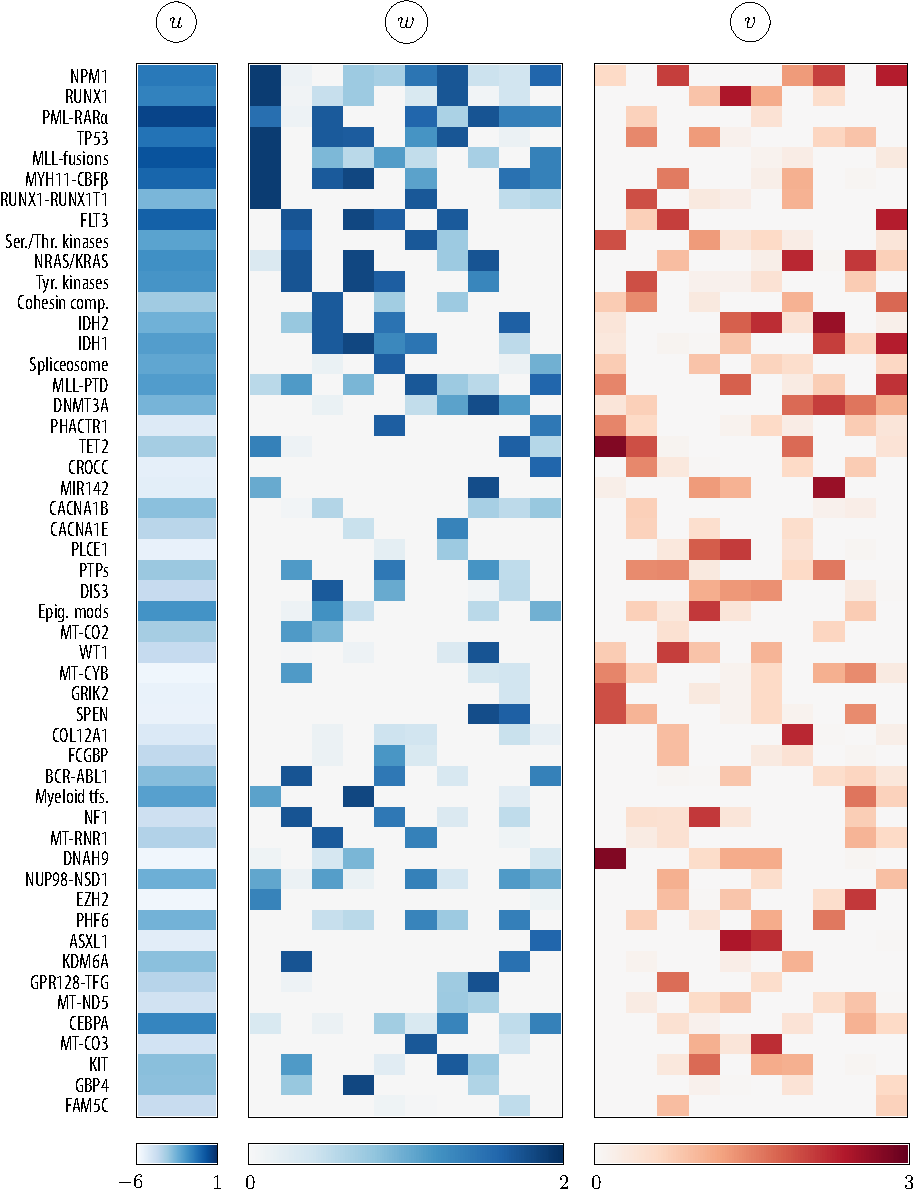
\includegraphics[width=\textwidth]{figures/genes/mat_aml.pdf}\\[2em]
\caption{Test}
\end{figure}

\begin{figure}[htb]
\centering
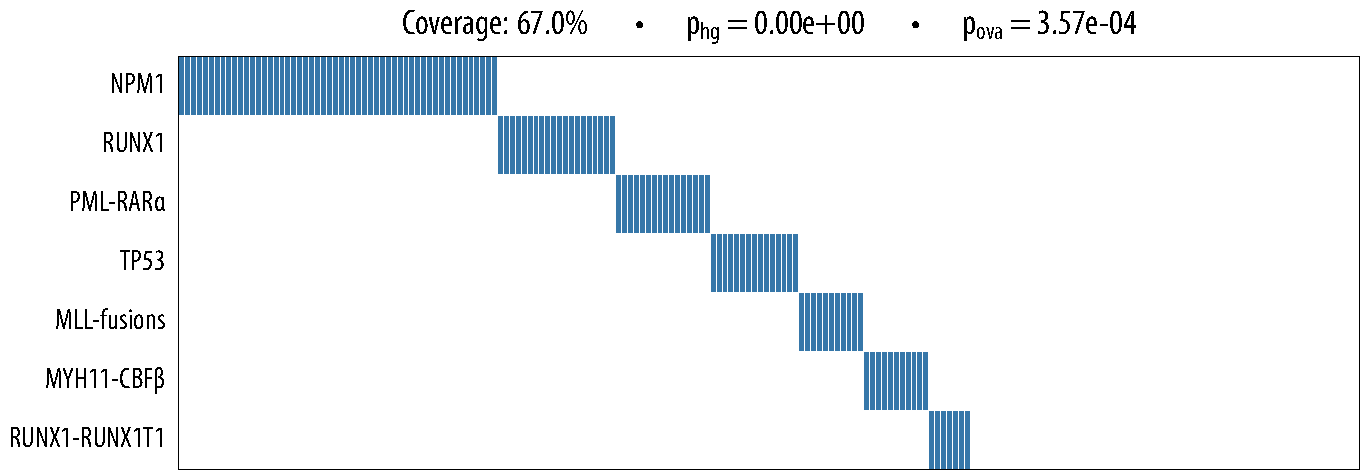
\includegraphics[width=\textwidth]{figures/genes/aml_1.pdf}\\[2em]
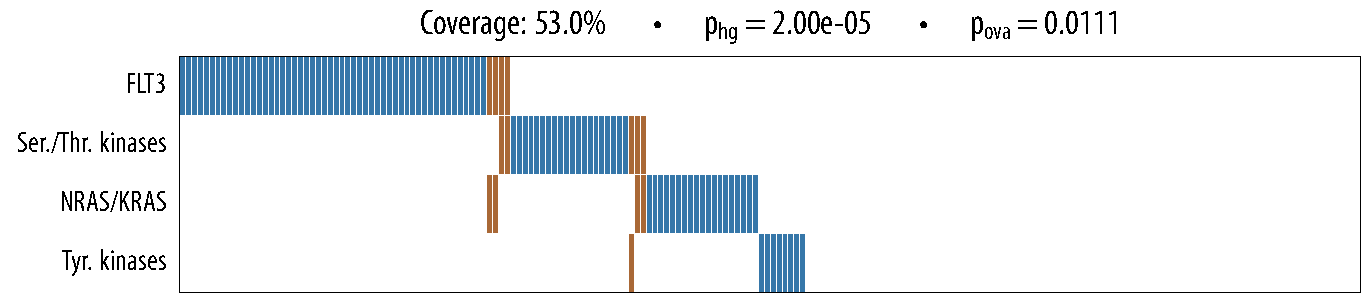
\includegraphics[width=\textwidth]{figures/genes/aml_2.pdf}\\[2em]
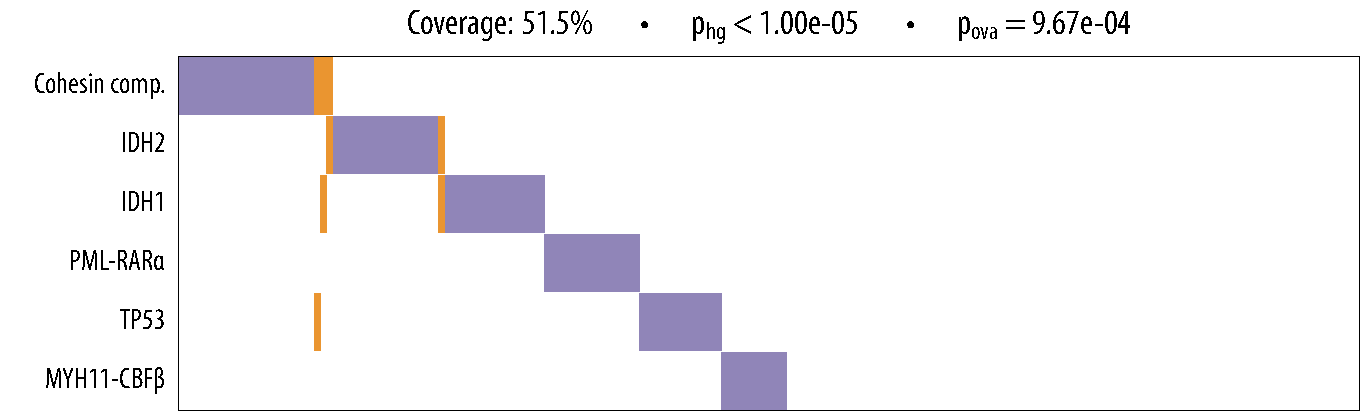
\includegraphics[width=\textwidth]{figures/genes/aml_3.pdf}\\[2em]
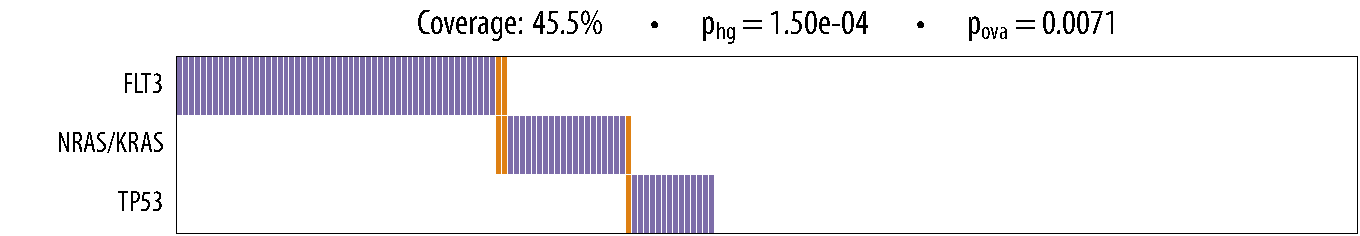
\includegraphics[width=\textwidth]{figures/genes/aml_4.pdf}\\[2em]
\caption{Test}
\end{figure}

\begin{figure}[htb]
\centering
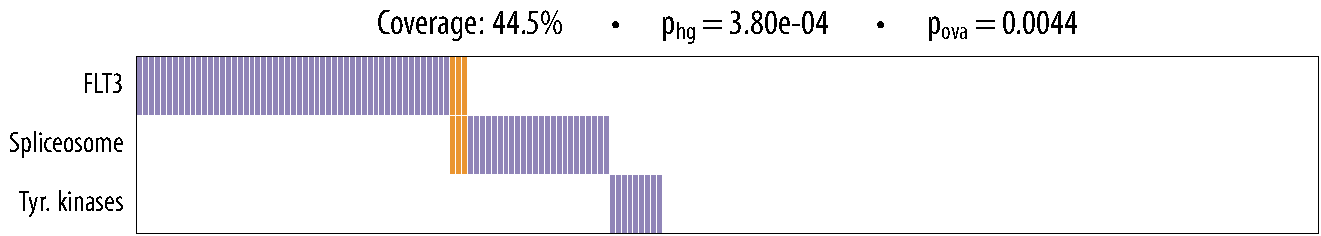
\includegraphics[width=\textwidth]{figures/genes/aml_5.pdf}\\[2em]
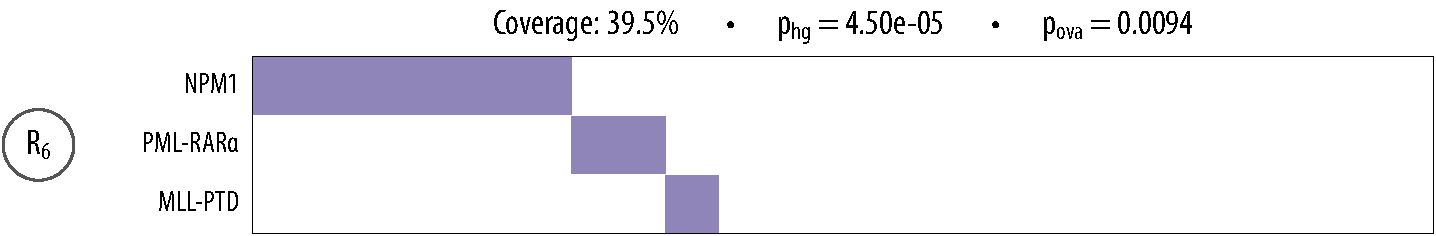
\includegraphics[width=\textwidth]{figures/genes/aml_6.pdf}\\[2em]
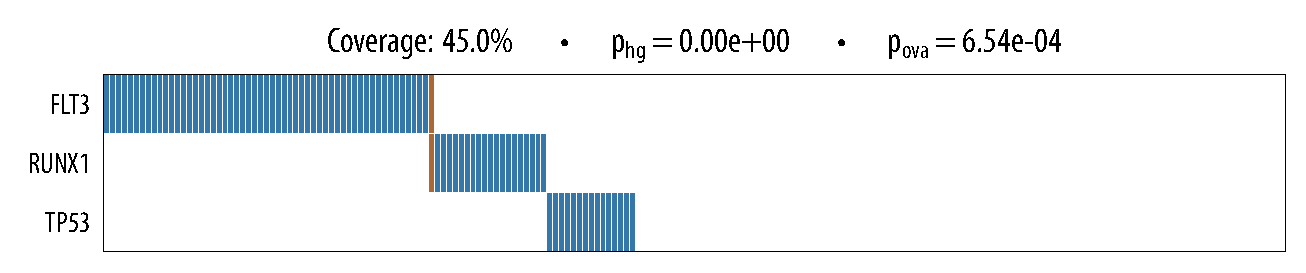
\includegraphics[width=\textwidth]{figures/genes/aml_7.pdf}\\[2em]
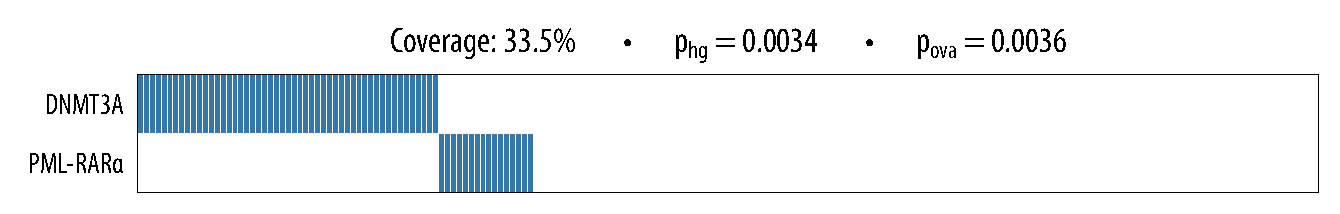
\includegraphics[width=\textwidth]{figures/genes/aml_8.pdf}\\[2em]
\caption{Test}
\end{figure}

\begin{figure}[htb]
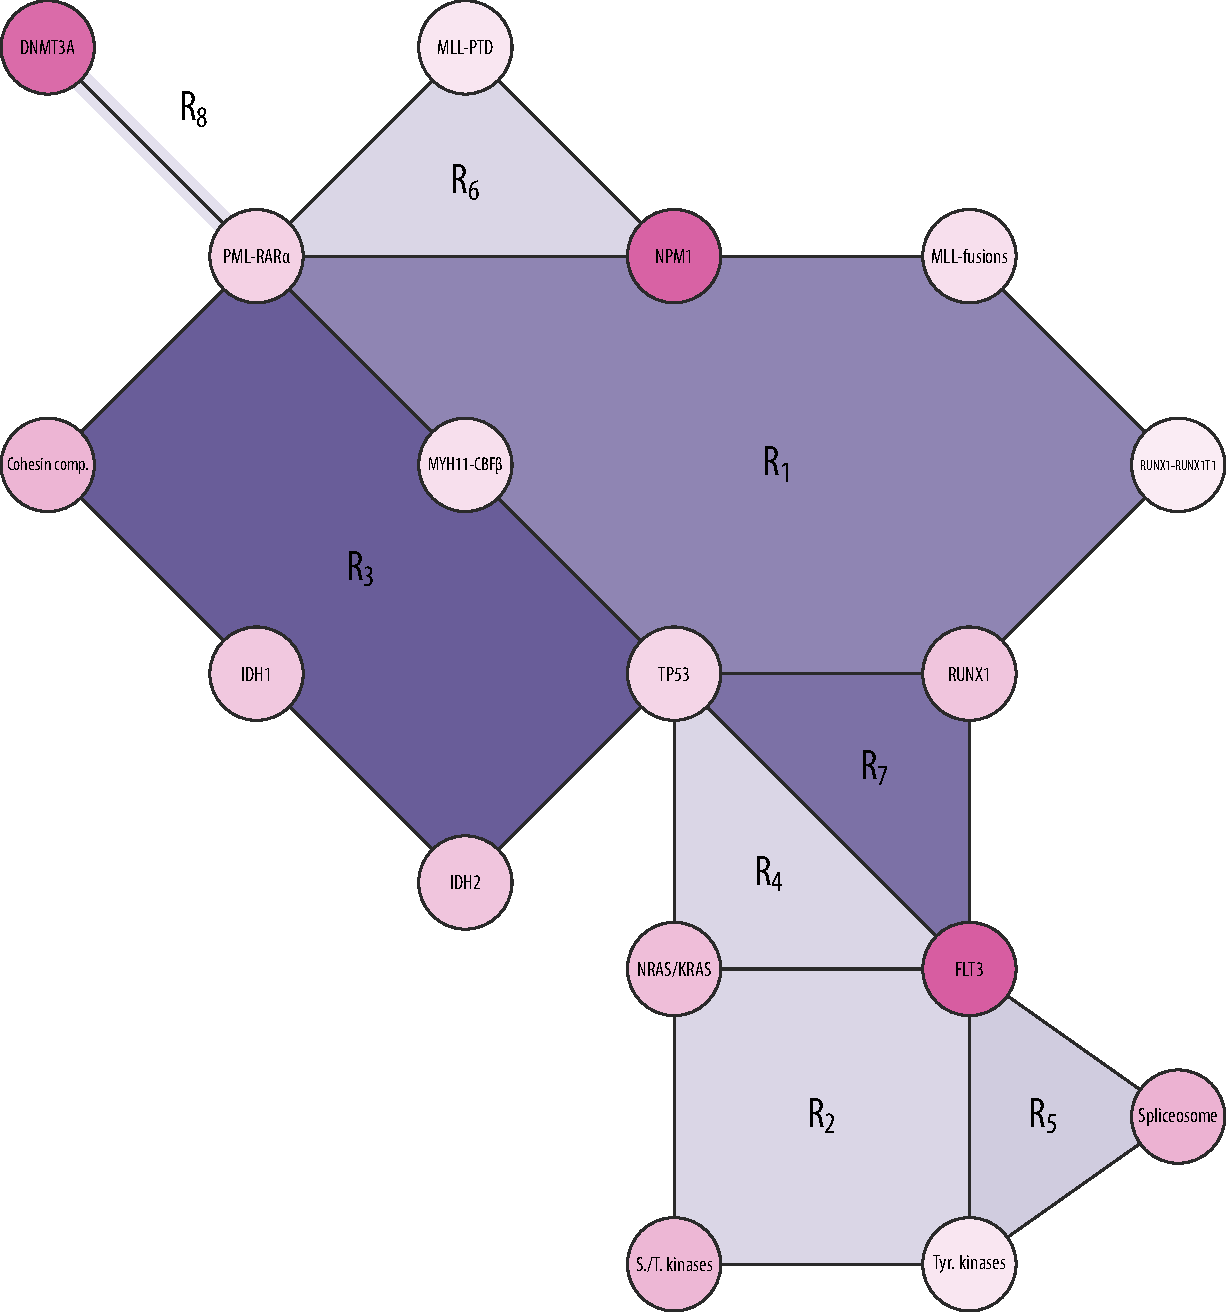
\includegraphics[width=\textwidth]{figures/genes/graph_aml.pdf}\\[2em]
\caption{AML repulsive graph}
\end{figure}

\begin{figure}[htb]
\centering
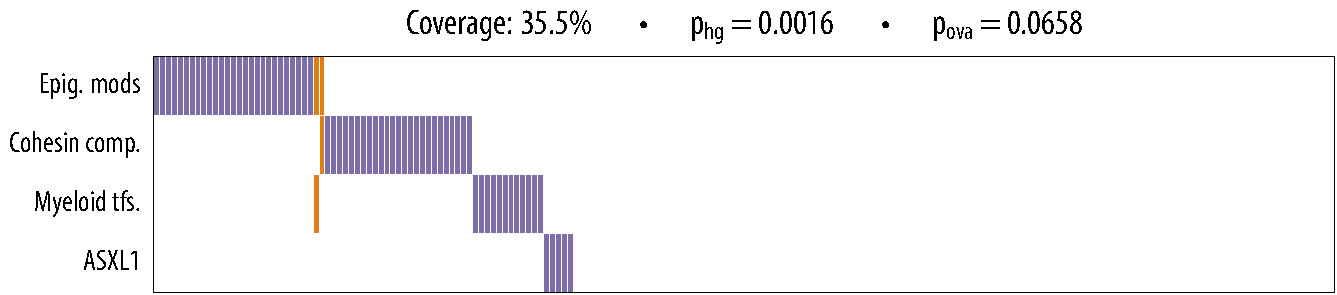
\includegraphics[width=\textwidth]{figures/genes/aml_comet1.pdf}\\[2em]
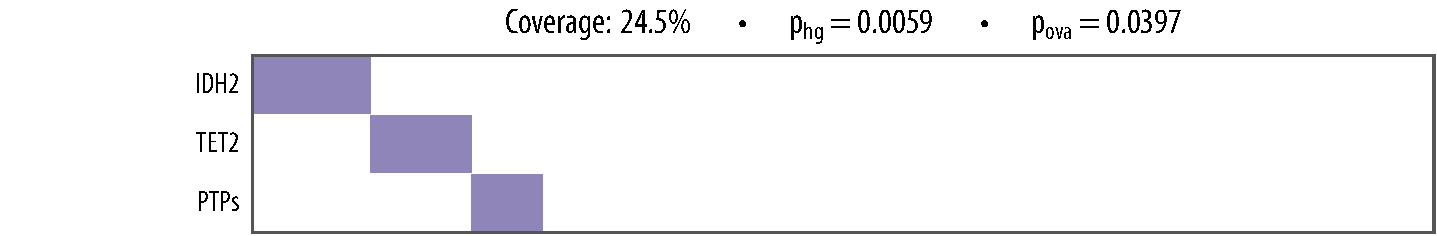
\includegraphics[width=\textwidth]{figures/genes/aml_comet2.pdf}\\[2em]
\caption{CoMEt extra groups (probably appendix)}
\end{figure}

\begin{figure}[htb]
\centering
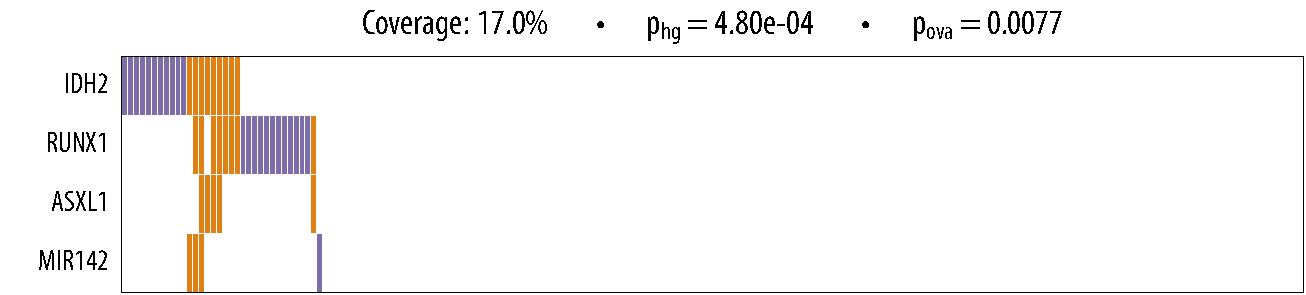
\includegraphics[width=\textwidth]{figures/genes/aml_2_a.pdf}\\[2em]
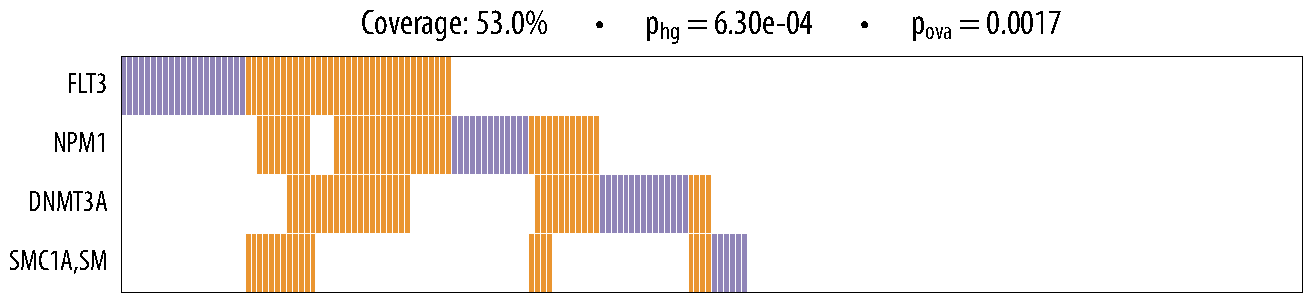
\includegraphics[width=\textwidth]{figures/genes/aml_1_a.pdf}\\[2em]
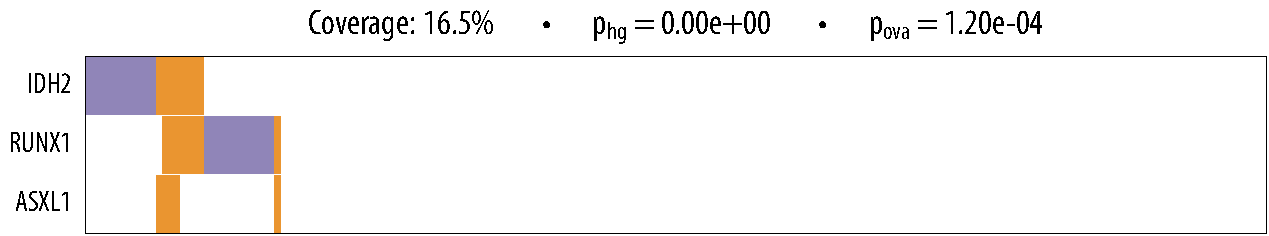
\includegraphics[width=\textwidth]{figures/genes/aml_3_a.pdf}\\[2em]
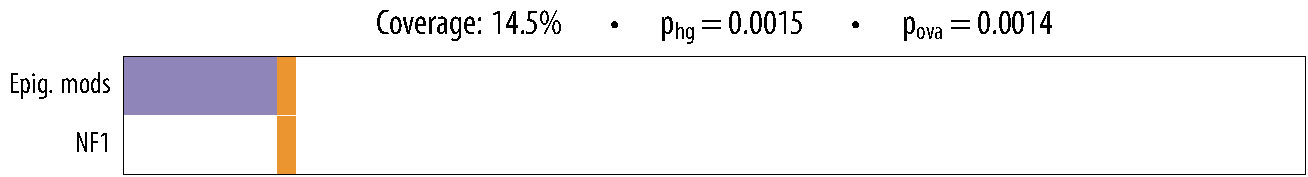
\includegraphics[width=\textwidth]{figures/genes/aml_5_a.pdf}\\[2em]
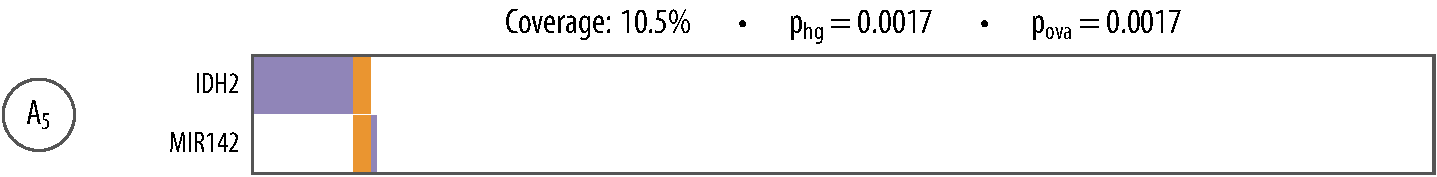
\includegraphics[width=\textwidth]{figures/genes/aml_4_a.pdf}\\[2em]
\caption{Test}
\end{figure}

\subsection{Breast cancer (BRCA)}
\begin{figure}[htb]
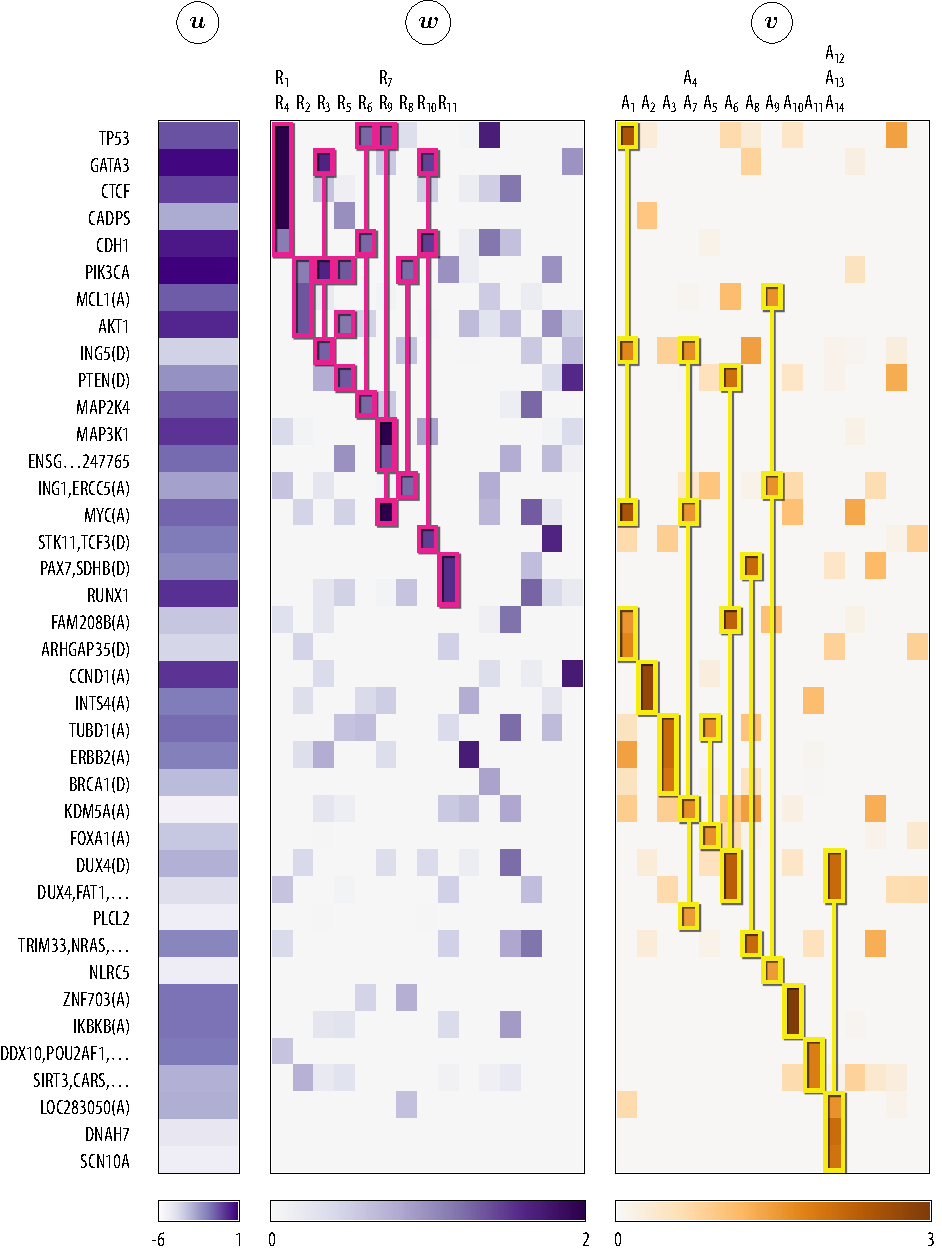
\includegraphics[width=\textwidth]{figures/genes/mat_brca.pdf}\\[2em]
\caption{Test}
\end{figure}

\begin{figure}[htb]
\centering
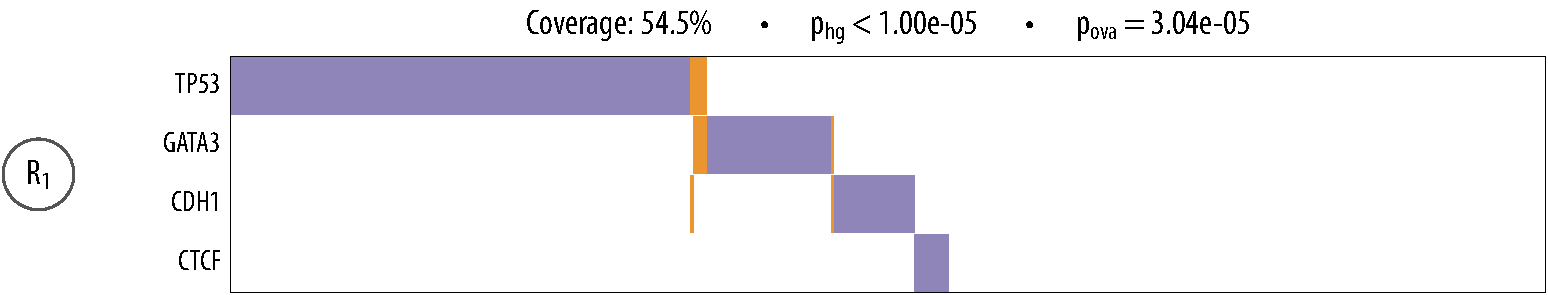
\includegraphics[width=\textwidth]{figures/genes/brca_1.pdf}\\[2em]
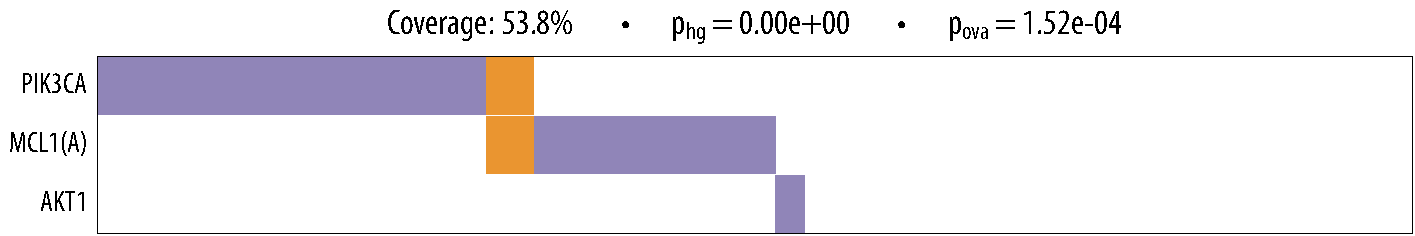
\includegraphics[width=\textwidth]{figures/genes/brca_6.pdf}\\[2em]
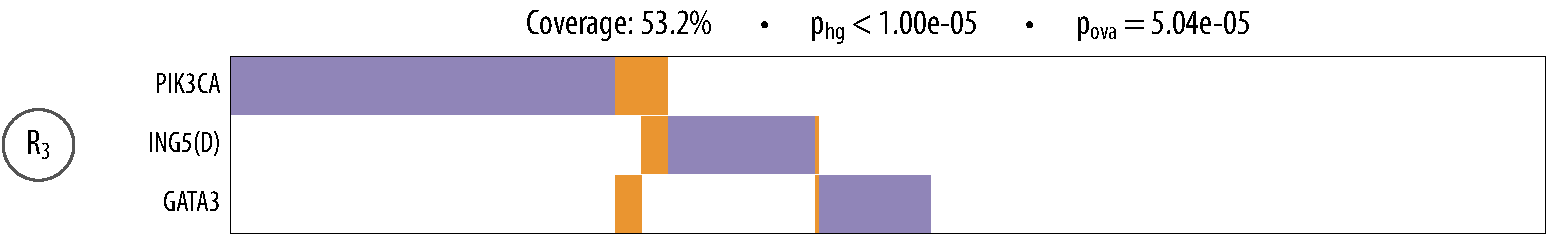
\includegraphics[width=\textwidth]{figures/genes/brca_8.pdf}\\[2em]
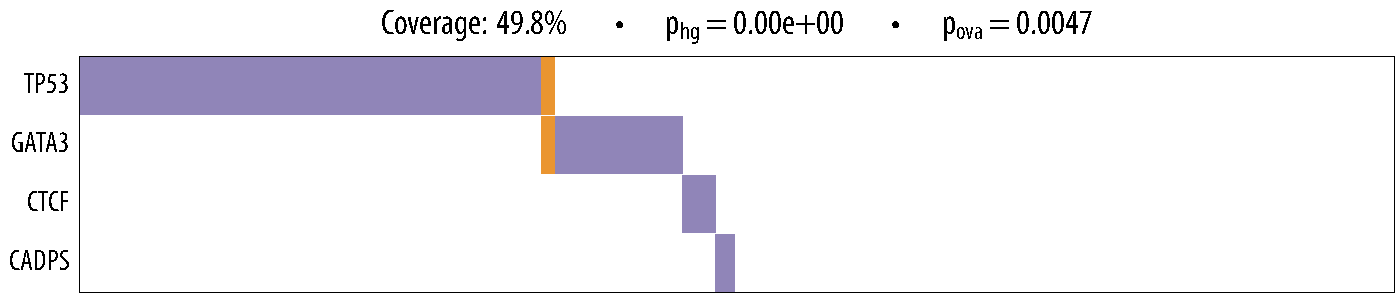
\includegraphics[width=\textwidth]{figures/genes/brca_2.pdf}\\[2em]
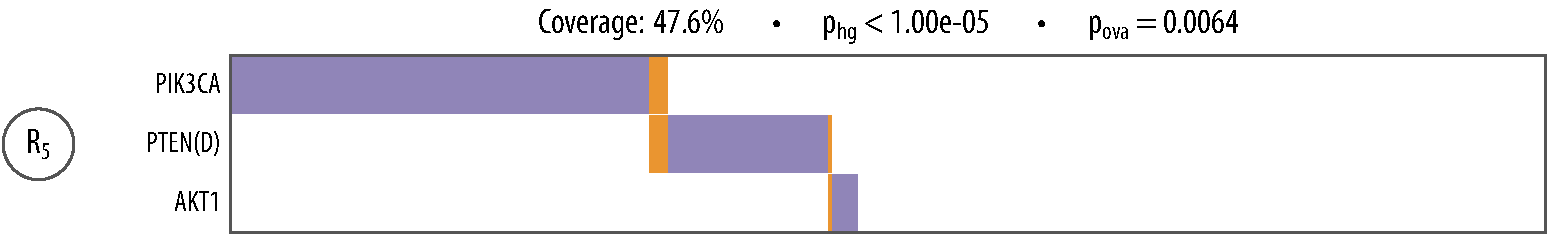
\includegraphics[width=\textwidth]{figures/genes/brca_5.pdf}\\[2em]
\caption{BRCA repulsive (I)}
\end{figure}

\begin{figure}[htb]
\centering
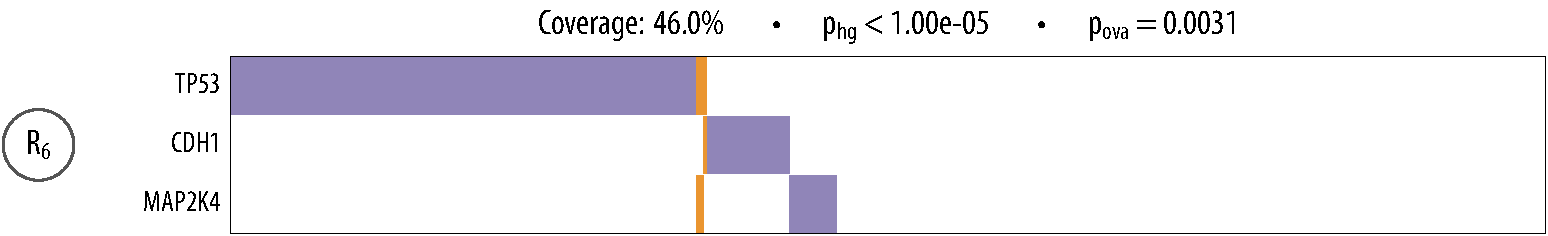
\includegraphics[width=\textwidth]{figures/genes/brca_4.pdf}\\[2em]
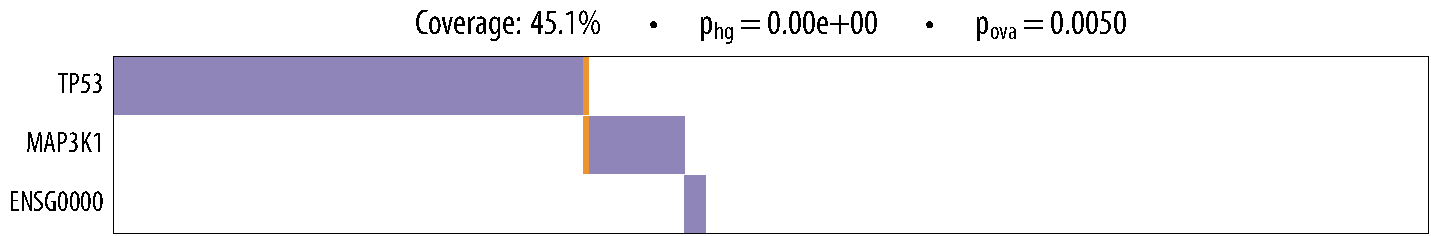
\includegraphics[width=\textwidth]{figures/genes/brca_3.pdf}\\[2em]
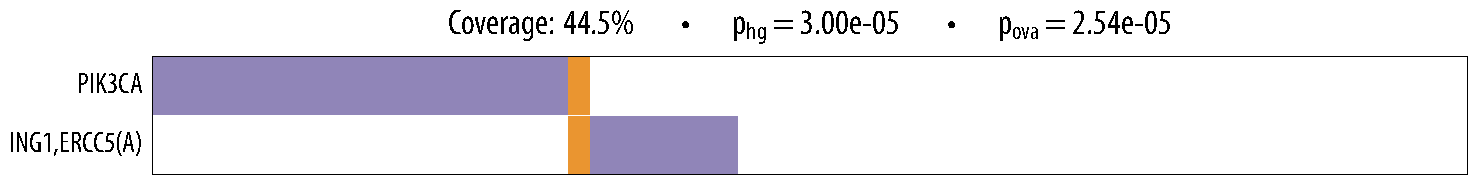
\includegraphics[width=\textwidth]{figures/genes/brca_11.pdf}\\[2em]
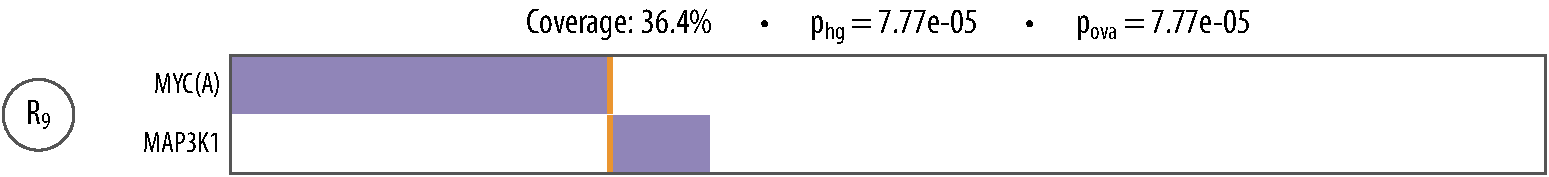
\includegraphics[width=\textwidth]{figures/genes/brca_10.pdf}\\[2em]
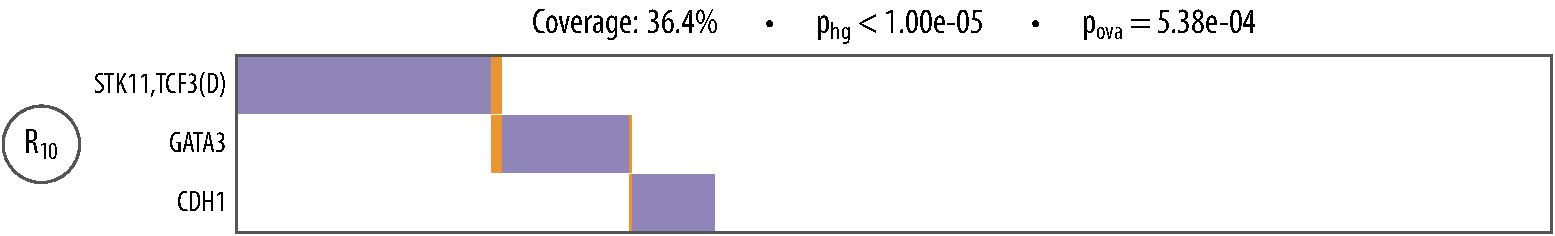
\includegraphics[width=\textwidth]{figures/genes/brca_7.pdf}\\[2em]
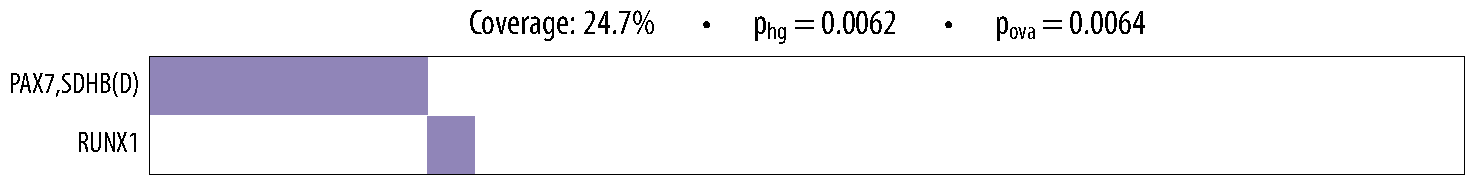
\includegraphics[width=\textwidth]{figures/genes/brca_9.pdf}\\[2em]
\caption{BRCA repulsive (II)}
\end{figure}

\begin{figure}[htb]
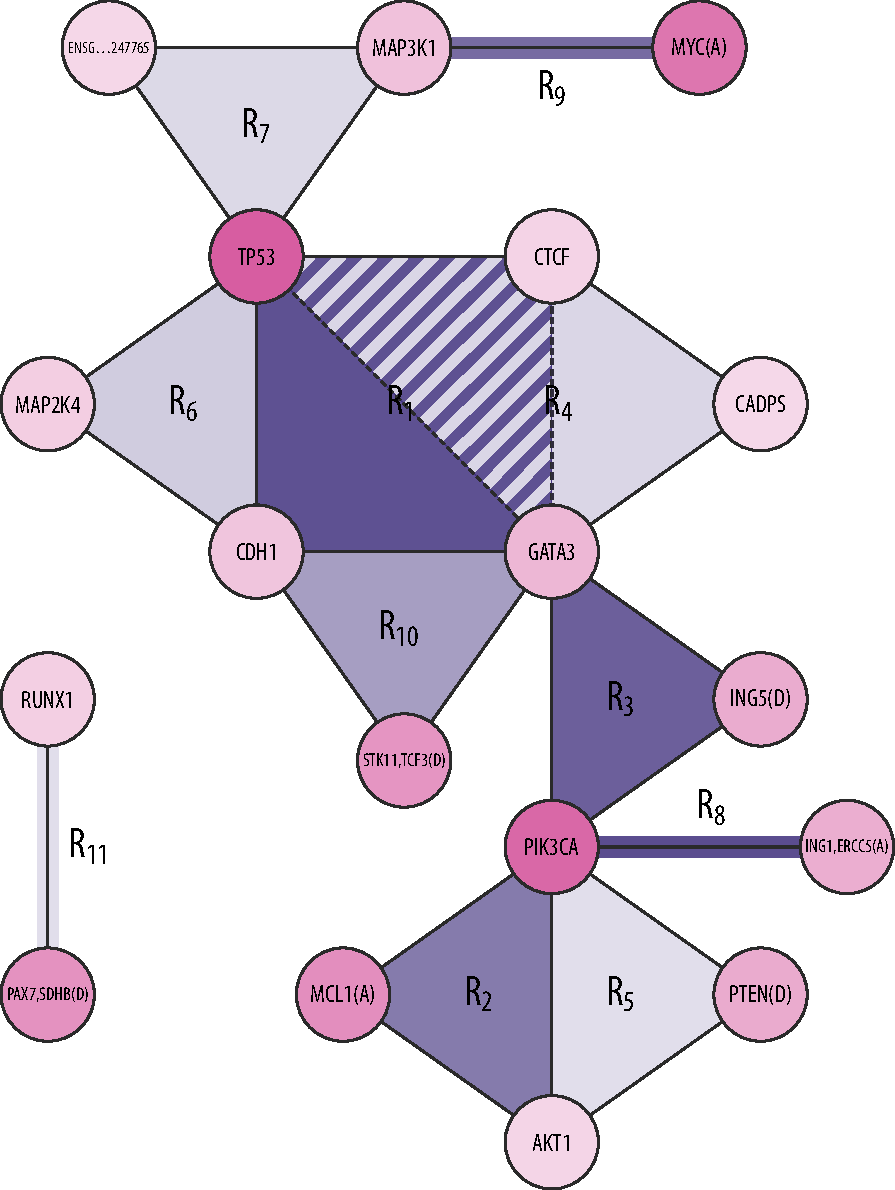
\includegraphics[width=\textwidth]{figures/genes/graph_brca.pdf}\\[2em]
\caption{BRCA repulsive graph}
\end{figure}

\begin{figure}[htb]
\centering
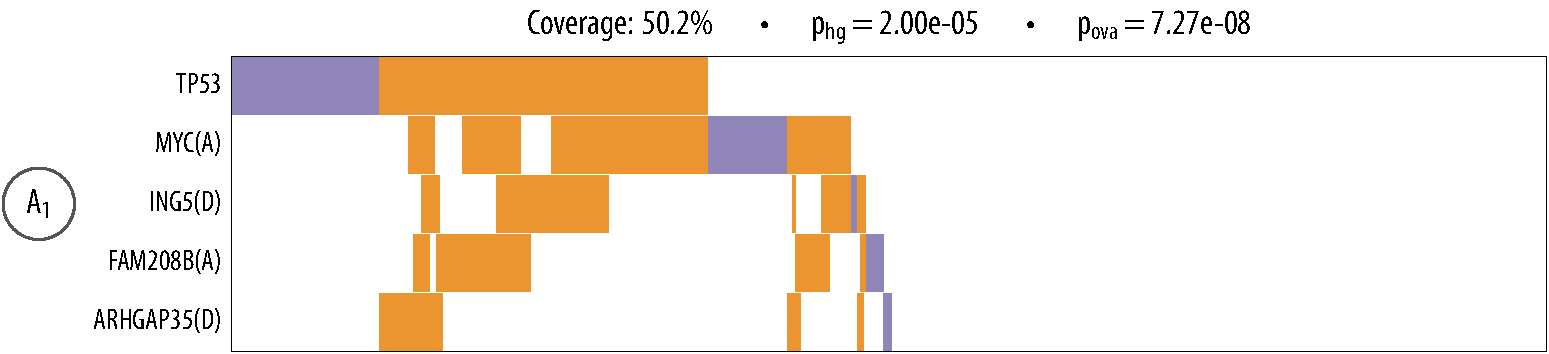
\includegraphics[width=\textwidth]{figures/genes/brca_1_a.pdf}\\[2em]
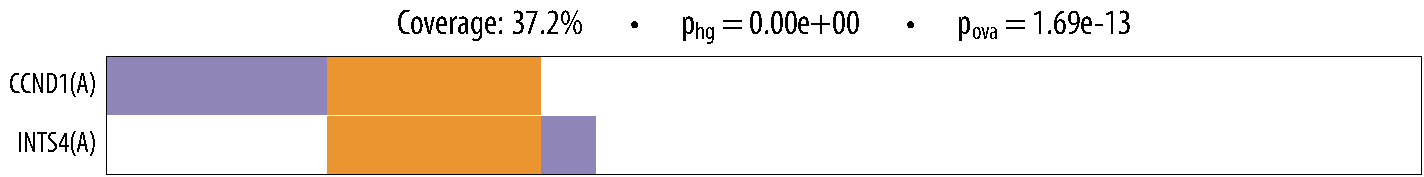
\includegraphics[width=\textwidth]{figures/genes/brca_11_a.pdf}\\[2em]
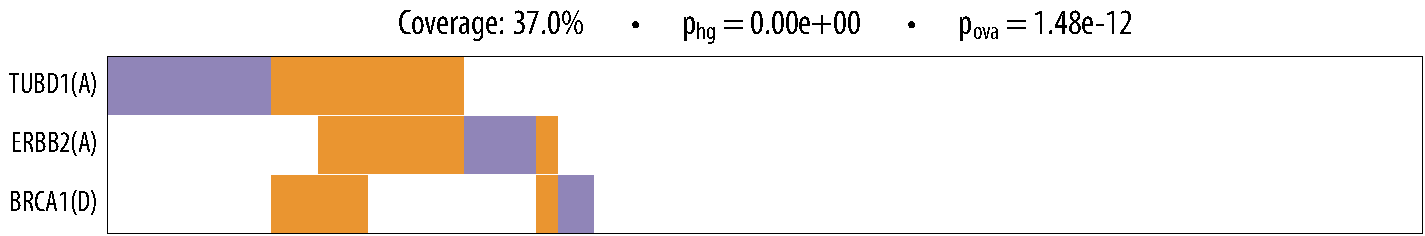
\includegraphics[width=\textwidth]{figures/genes/brca_7_a.pdf}\\[2em]
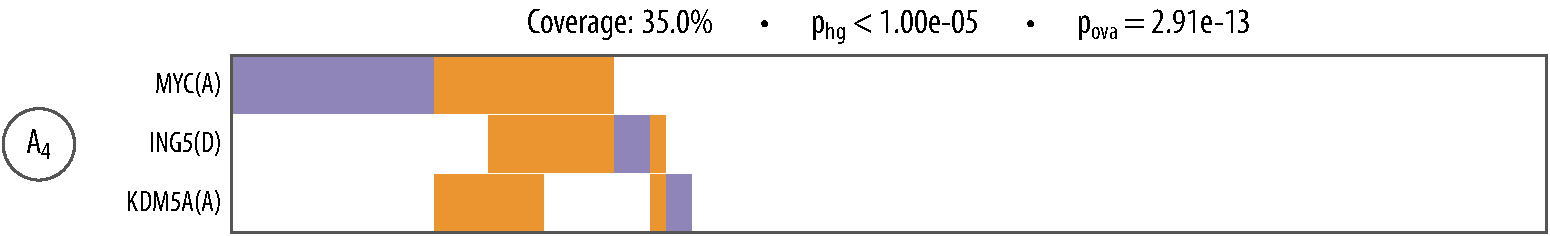
\includegraphics[width=\textwidth]{figures/genes/brca_8_a.pdf}\\[2em]
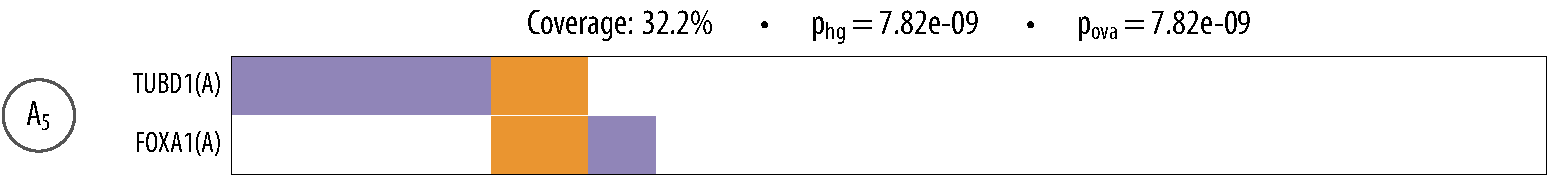
\includegraphics[width=\textwidth]{figures/genes/brca_14_a.pdf}\\[2em]
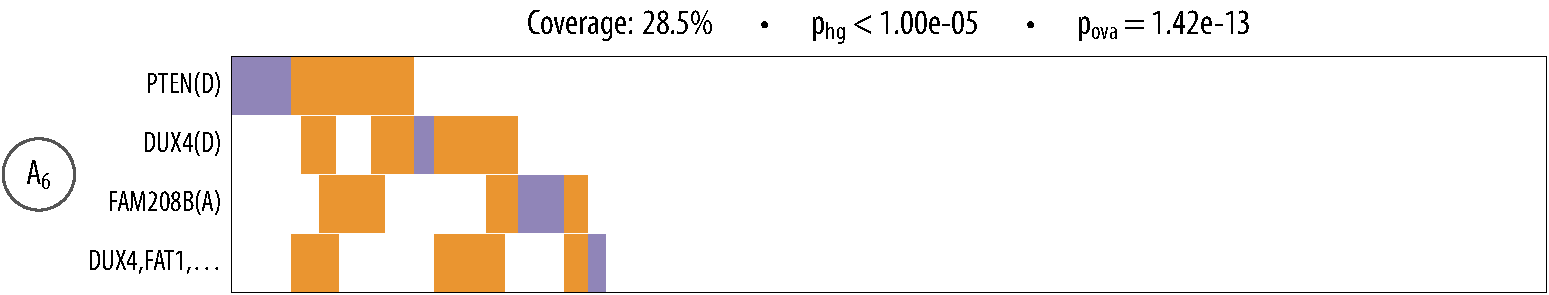
\includegraphics[width=\textwidth]{figures/genes/brca_4_a.pdf}\\[2em]
\caption{BRCA attractive}
\end{figure}

\begin{figure}[htb]
\centering
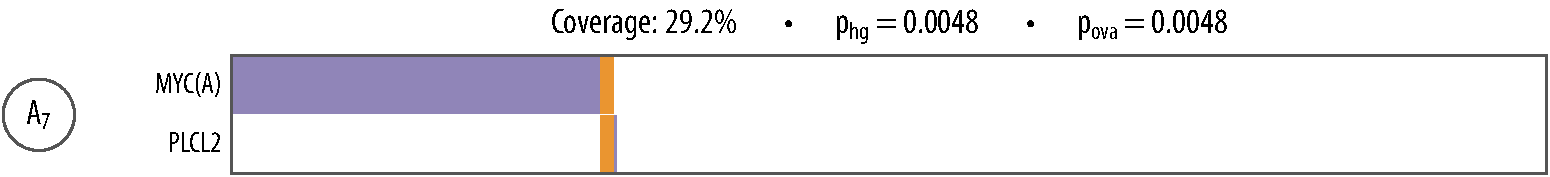
\includegraphics[width=\textwidth]{figures/genes/brca_9_a.pdf}\\[2em]
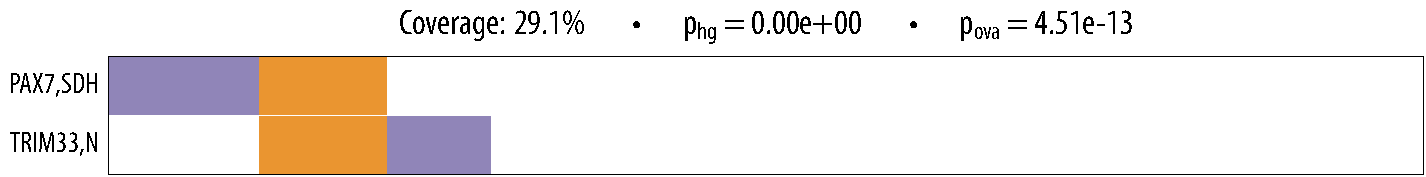
\includegraphics[width=\textwidth]{figures/genes/brca_13_a.pdf}\\[2em]
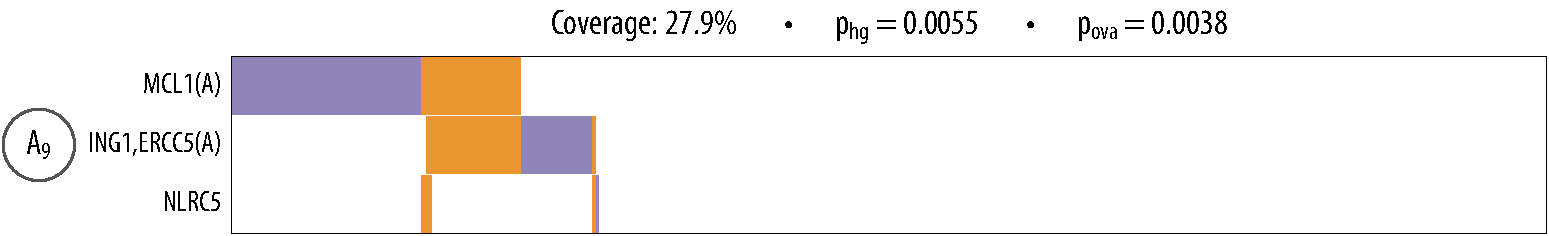
\includegraphics[width=\textwidth]{figures/genes/brca_5_a.pdf}\\[2em]
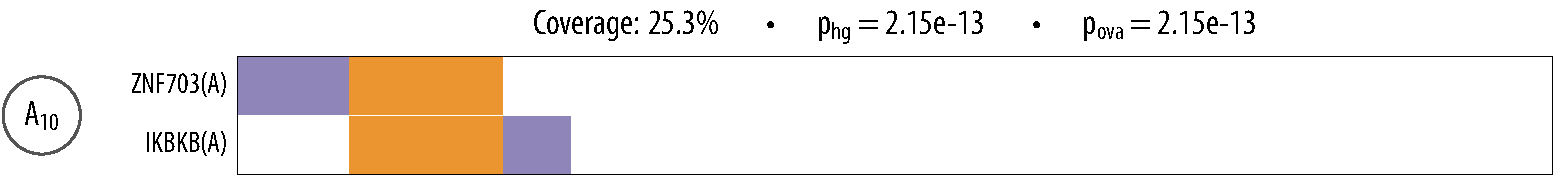
\includegraphics[width=\textwidth]{figures/genes/brca_10_a.pdf}\\[2em]
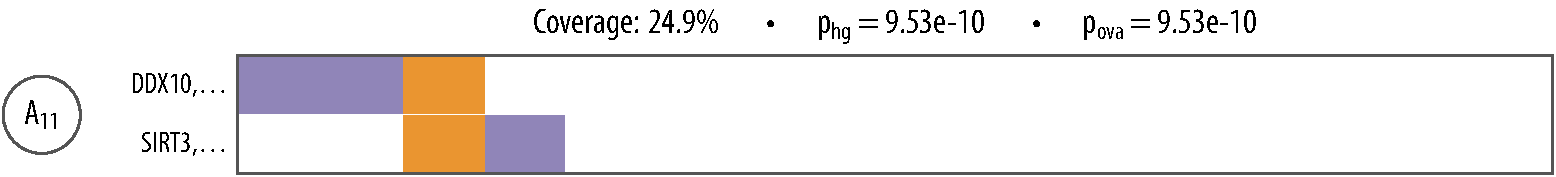
\includegraphics[width=\textwidth]{figures/genes/brca_12_a.pdf}\\[2em]
\caption{BRCA attractive (appendix I)}
\end{figure}

\begin{figure}[htb]
\centering
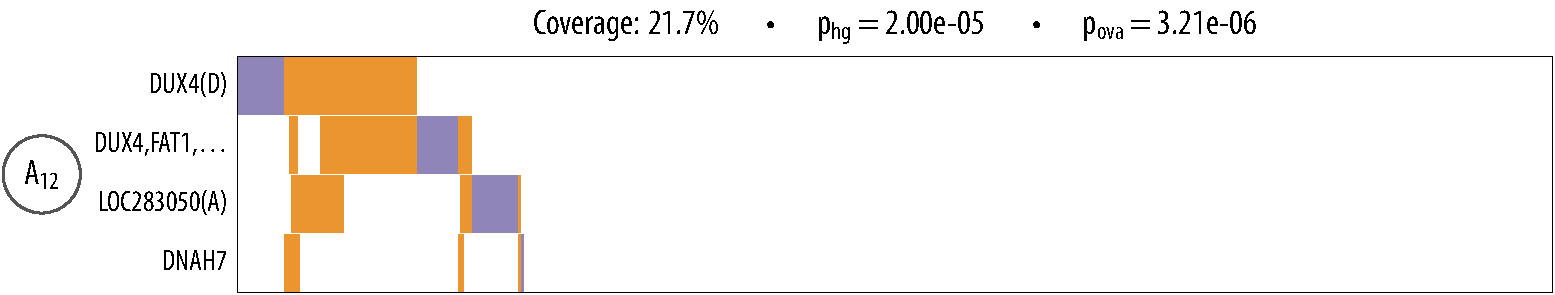
\includegraphics[width=\textwidth]{figures/genes/brca_3_a.pdf}\\[2em]
%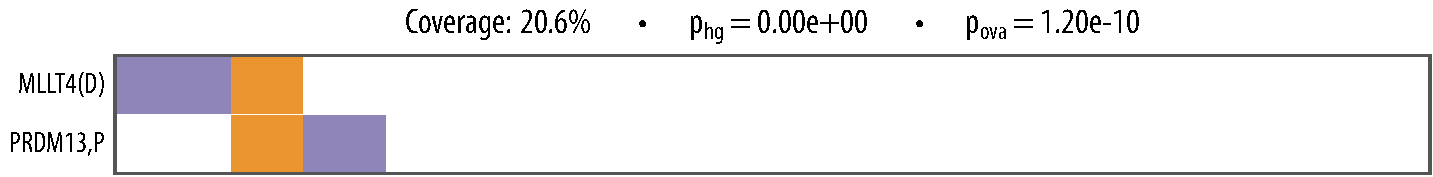
\includegraphics[width=\textwidth]{figures/genes/brca_15_a.pdf}\\[2em]
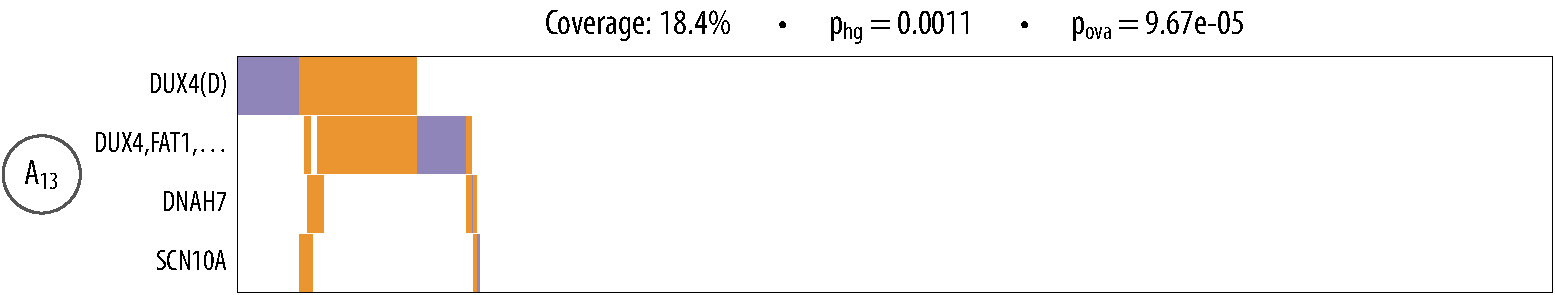
\includegraphics[width=\textwidth]{figures/genes/brca_2_a.pdf}\\[2em]
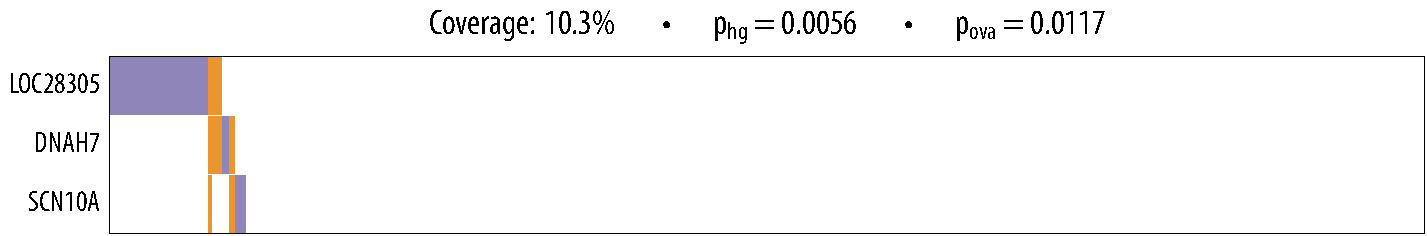
\includegraphics[width=\textwidth]{figures/genes/brca_6_a.pdf}\\[2em]
\caption{BRCA attractive (appendix II)}
\end{figure}

\section{Conclusion}